\chapter{Introduction}
\label{Chap:intro}

% epigraph
\setlength{\unitlength}{1pt}
\setlength{\epigraphwidth}{11cm}
\epigraph{What is a stupid question? If there is only one answer to the question instead of other possibilities, it is a stupid question. \cite{cheung1988}}{--- Steven N. S. Cheung\\ \textit{Way of thinking (1984)}}

% introduction and purpose (done 2021年7月9日14:34:47)
The world is made up of various substances, and even the same substance can be in different \textit{phases}. Besides finding new particles and materials, discovering new phases of matter is also an essential subject of physics. When discovered phases of matter accumulating, how to classify, explain and understand them from the perspective of microscopic theory gradually becomes the core topic of physics. This thesis will introduce a new quantum phase of ultracold atoms, i.e. the quantum liquid droplet. It is originated from the famous beyond mean-field correction of the Bose-Einstein condensate (BEC), i.e. the Lee-Huang-Yang (LHY) correction\cite{lee1957}, which will be discussed detailedly in the latter chapters. This chapter will introduce the history of the topic developed in recent years and its influence on other fields. I try to offer readers a broader picture for a better understanding of quantum liquid droplet.

% arrangement of this chapter (done 2021年7月9日14:34:24)
This chapter is arranged as follows: section \ref{sec:intro-background} introduces our research goal, the quantum droplet. By introducing some background knowledge and researches from related fields, I try to discuss why we study the Na-Rb BEC-mixture droplet. Section \ref{sec:intro-LHY} will discuss the core concepts of LHY correction and its history, as a precursor of Chapter \ref{Chap:theory}. Finally, section \ref{sec:intro-outline} offers the arrangement of the whole thesis.

\section{Why quantum liquid droplets?}
\label{sec:intro-background}

% start from classical droplet (done 2021-10-26 23:57:25)
Before answering the question on the title, i.e. about the \textit{quantum} liquid droplet, we first draw some attention to the \textit{classical} liquid-gas phase transition. As shown in Fig. \ref{Classical_and_quantum_droplet}, a classical gas can be regarded as a bunch of interacting particles. Typically, we use the Van der Waals interaction as a good approximation, i.e. a hard-core (repulsion) plus an attractive long-range potential. By adding this inter-particle interaction to the equation of state, we get the famous Van der Waals equation:
\begin{equation}
\label{VdW equation}
(P+a\frac{n^2}{V^2})(V-bn)=nRT
\end{equation}
where the ``\(b\)'' factor represents the hardcore size, since the effective volume of sample is enlarged, and ``\(a\)'' shows the attractive interaction between particles which reduces the pressure of the sample. This equation implies the liquid-gas phase transition when the temperature is lowering down to a specific \(T_C=\frac{8a}{27Rb}\). The detailed analysis could be found in the textbook \cite{Cowan2005}. So, here we only focus on the physics picture. For a liquid phase sample, as shown in Fig. \ref{Classical_and_quantum_droplet} right-top panel, the particles are squeezed to their hard-cores touching to each other. This features the incompressibility of a liquid sample. The kinetic energy of particles maintain their mobility, and due to easily exchange of particle position, we still have a fluid instead of a solid phase. In another perspective, the attractive range of particles overlapping with each other indicates a strong correlation. One particle could affect many other particles. We call this a long-range interaction system, which is typically hard to tackle. So, even with full knowledge of its microscopic equation, sometimes the behaviour of liquid can still amaze us, such as Non-Newtonian fluid or liquid crystal.

% add classical and quantum droplet comparison figure (done: 2021年7月29日19:30:32)
\begin{figure}[htbp]
\begin{center}
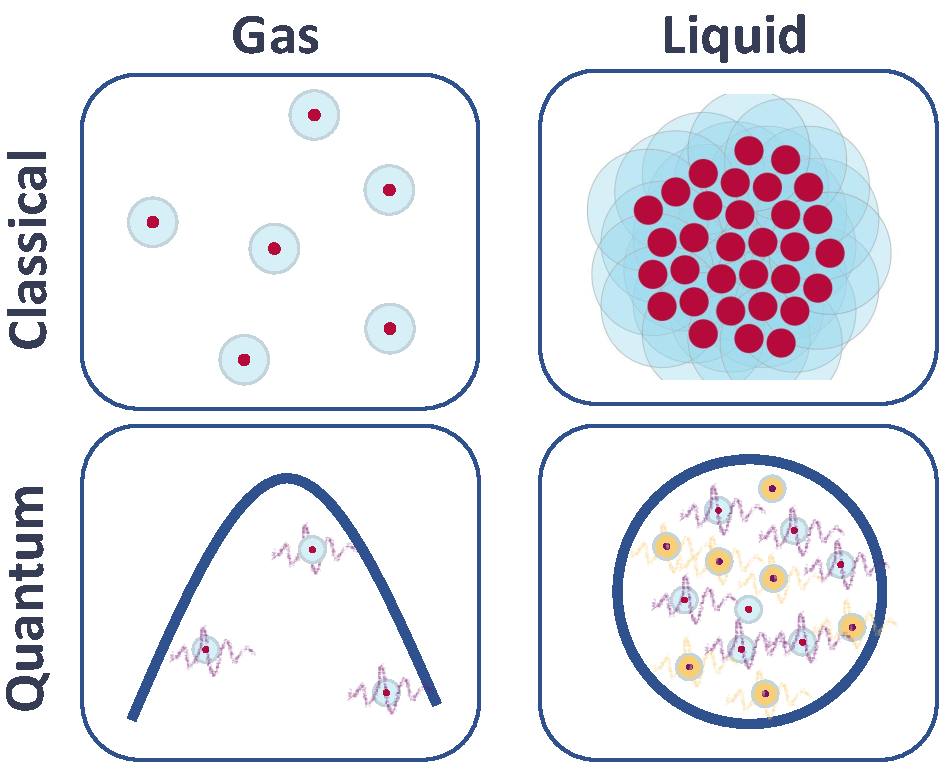
\includegraphics [width = 0.8 \linewidth]{Classical_and_quantum_droplet.pdf}
\end{center}
\caption[Comparison between classical and quantum liquid droplet]{Classical and quantum Liquid-gas phase transition. The upper panel shows a classical liquid-gas phase transition, explained by the famous Van der Waals equation. With this theory, particles interact with short-range hardcore (red solid part) and long-range attraction (light-blue outer). When the temperature lowers to the critical temperature, the sample undergoes a phase transition to be a liquid. As shown in the upper-right block, particles stay close to each other with inter-particle distance around the size of its hardcore. Meanwhile, their long-range parts overlap, showing a strongly correlated feature. For the lower panel, we draw the quantum liquid-gas phase transition for a BEC mixture sample. The thick blue line represents the shared wave function for the condensate part. The particle with a de-Broglie wave-packet represents the quantum depletion due to interaction excitation from the condensate. The right-bottom one shows the BEC mixture liquid droplet, which is the main topic of this thesis.}
\label{Classical_and_quantum_droplet}
\end{figure}

% to quantum matter, quantum gas sample (done: 2021年8月16日21:54:08)
Then, a question arises naturally for cold atom physicists: what about a quantum system? Is there any liquid phase for a Bose-Einstein condensate? A positive answer is provided by Petrov in 2015 \cite{petrov2015}. For a dilute ultracold BEC mixture, we do have a liquid phase. However, this kind of liquid is dramatically different from the classical one. First, it is a zero-temperature sample, which means the thermal fluctuation is suppressed. Second, the sample is still dilute with an interparticle distance larger than 100 nm (interacting range typical around several nm). This indicates the system should be still in a weak-interacting case. Finally, quantum fluctuation shows its essential role. However, instead of serving as a driven force for mobility, the quantum fluctuation cures the sample's collapse or implosion. To study this sample, we could understand more profound the beyond mean-field correction of this many-body system.

% introduce quantum depletion and call droplet (done 2021年7月26日17:53:24)
As a new topic in ultracold atoms, quantum liquid droplets originated from the deep understanding of the beyond mean-field theory of Bose-Einstein condensate (BEC) and from an innovative and careful extrapolation of textbook theory. In the past 25 years discovery of ultracold gases, mean-field theory (MF theory), as the zero-order solution of a many-body system, dominates the explanation of most phenomena. Especially for Bose-Einstein condensate, it explains plenty of interesting experiment observations, including the state of the equation for in-trap sample, excitation mode, dark soliton, bright solution, BEC collapse and so on. This zero-order approximation considers the condensates as a single wave-function \(\Psi\), which is based on the observation that most atoms share the same ground state, i.e. the \(k=0\) state (for uniform case). However, particles from the condensate could be excited to a finite momentum state due to the interaction between particles. From the microscopic theory of condensate, these particles with \(k>0\) have a fraction of order of \(\sqrt{na^3}\) compared to the condensate part, which occupies a tiny portion when the interaction is weak. Thus, we call it quantum depletion. This tiny portion brings only a tiny correction to its ground-state energy; so, people typical ignore its effect in most cases. However, things get incredibly different in the quantum liquid droplet; here, quantum depletion plays a vital role because the depletion part contributes a competitive energy scale to the mean-field energy. 

% what is quantum droplet? (done 2021年7月26日21:44:05)
Proposed by Petrov in 2015 \cite{petrov2015}, a BEC mixture with overall negative mean-field energy could survive from collapsing and form a quantum droplet. Surprisingly, this theory was first used to explain the self-bound behaviour in the dipolar gas \cite{ferrier2016Liquid,chomaz2016}. Then in 2018, Leticia group \cite{cabrera2018quantum} discovered the first double BEC droplet in a spin mixture of \(^{39}\)K. These two distinctive systems are related to the same theoretical explanation, showing the ubiquity that how important role for the LHY correction in ultracold atoms. For both cases, the mean-field energy approaches zero and is tuned by a Feshbach resonance for an inter-species \(s\)-wave contact interaction. Meanwhile, the LHY correction remains a positive value and grows even fast than the mean-field one when the density of the sample increasing. So, it cures the mean-field collapse. The difference between a dipolar droplet and a mixture BEC droplet is the inter-particle interaction type: for dipolar case, the interaction is anisotropic, which renders an anisotropic sample as well; however, for the BEC mixture case, thanks to the isotropic interaction, the sample shows a perfect spherical shape.

% droplet in different system (done: 2021年8月15日11:40:20)
As mentioned before, Petrov's theory was first used to the dipolar droplet \cite{ferrier2016Liquid,chomaz2016}, which is made of magnetic atoms with anisotropic interaction. Then in 2018, two groups \cite{cabrera2018quantum,semeghini2018self} produced the double BEC droplet exactly matching Petrov's original proposal. Latter, many works sprung up, in both experiment and theory. Leticia's group produce the droplet in a wave-guide \cite{cheiney2018bright}, in which they study the bright soliton to the droplet phase transition. From the low-dimension point of view, many theoretical proposals are developing, including \cite{petrov2016ultradilute,Ilg2018,Cui2021}. In another point of view, i.e. the gas phase sample with near-zero mean-field energy, theory \cite{Jorgensen2018}, and experiment \cite{skov2020} study the changing of monopole mode of an LHY gas. 

% why we study droplet? (done: 2021年8月15日19:44:00)
The initial purpose of our research was to make a heteronuclear droplet. With a rough calculation, we estimate its lifetime could reach about 100 ms, enabling us to do further research such as its excitation spectrum and the self evaporation. However, later we find the lifetime of the sample limited to 10 ms level. We attribute this to the large three-body loss between two species. Then, we have to turn our research goal to study the LHY effects in a double BEC of $^{23}$Na and $^{87}$Rb atoms in two different ways. First, we build the heteronuclear quantum liquid droplet in free space with more than $10^4$ atoms when the interspecies Na-Rb scattering length is tuned into the mean-field collapse regime. Under optimized conditions, a low-number-density droplet with a lifetime exceeding the observation time is observed. We also investigate the liquid-to-gas phase transition and obtain the critical atom numbers at the phase boundary. Second, we measure the release energies of two types of gas-phase mixtures, the pure in-trap gas and the gas formed after a droplet crosses the liquid-to-gas transition, and observe their opposite dependence on the interaction strength.  With calculations based on extended Gross-Pitaevskii equations (eGPEs), our results confirm the crucial contribution of $E_{\rm LHY}$ and its effects in stabilizing the heteronuclear double BEC far into the mean-field collapse region.

\section{Quantum depletion and LHY correction}
\label{sec:intro-LHY}

% Why discuss quantum depletion here (done 2021年8月17日13:20:01)
Back to the motivation of studying quantum droplets, the essential ingredient is the beyond-mend-field effect in a Bose condensate,i.e. the Lee-Huang-Yang (LHY) correction. LHY correction was first introduced by Lee, Huang and Yang in 1957~\cite{lee1957}, as the first-order correction of the ground state of Bose-Einstein condensate. However, due to its minor contribution, we typically can ignore it. However, when the zero-order mean-field energy is approaching zero, which means the LHY correction could compare to the MF energy or even dominant the sample, we need to treat it more seriously. This section introduces the quantum depletion and LHY correction as a precursor for the next chapter, which discusses the complete theory for the quantum droplet.

% quantum depletion and LHY correction (done 2021年8月17日13:24:47)
Let us consider a Bose-Einstein condensate, with its Hamiltonian as
\begin{equation}
H=\sum_k\epsilon_k\hat{a}_k^\dagger\hat{a}_k+\frac{g}{2V}\sum_{\left\{k_i\right\}}\hat{a}_{k_1}^\dagger\hat{a}_{k_2}^\dagger\hat{a}_{k_3}\hat{a}_{k_4}
\end{equation}
where $\epsilon_k$ is the kinetic energy for particles with momentum $k$, $hat{a}_k$ and $hat{a}_k^\dagger$ are creation and annihilation operator, $g$ as the interaction strength and $V$ is the total volume the whole system takes up.
By separating the condensate part and quantum fluctuation part, i.e. considering $a_0$ as $\sqrt{N}$ and write it away from other creation operators (with $k>0$), we have
\begin{equation}
\begin{split}
H=\frac{g N^2}{2V}&+\sum_{k\neq0}\left(\epsilon_k+gn_0\right)\hat{a}_k\dagger\hat{a}_k+\frac{gN}{2V}\sum_{k\neq0}\left(\hat{a}_k^\dagger\hat{a}_{-k}^\dagger+\hat{a}_k\hat{a}_{-k}\right)\\
&+\frac{g\sqrt{N}}{2V}\sum_{k_1+k_2+k_3=0}\left(\hat{a}_{k_1}^\dagger\hat{a}_{k_2}^\dagger\hat{a}_{k_3}+\hat{a}_{k_1}^\dagger\hat{a}_{k_2}\hat{a}_{k_3}\right)+\frac{g}{2V}\sum_{k_i\neq0}\hat{a}_{k_1}^\dagger\hat{a}_{k_2}^\dagger\hat{a}_{k_3}\hat{a}_{k_4}
\end{split}
\end{equation}
Ignore the higher order parts and do the Bogoliubov transition, we can get the diagonalized Hamiltonian as
\begin{equation}
\begin{split}
H\simeq \frac{g N^2}{2V}-\frac{1}{2}\sum _{k\neq 0} \left(\epsilon _k+\frac{g N}{V}-E_k\right)+\sum _{k\neq 0} E_k\hat{\alpha }_k^\dagger\hat{\alpha}_k\\
E_k=\sqrt{\epsilon_k\left(\epsilon_k+\frac{2gN}{V}\right)}=\sqrt{\frac{\hbar^2k^2}{2m}\left(\frac{\hbar^2k^2}{2m}+\frac{2gN}{V}\right)}
\end{split}
\end{equation}
The first part shows the energy shift (MF shift) for the condensate part. Second part shows summation of the energy of all particles with $k>0$, i.e. the quantum depletion. Third part shows the excitation spectrum of the sample and $E_k$ offers the dispersion of the sample. Now, we only consider the ground state properties, i.e. only consider the first two terms of the Hamiltonian. The fraction of depleted particle is
\begin{equation}
\frac{n_{\text{dp}}}{n}=\frac{8}{3\sqrt{\pi }}\sqrt{n a_s^3}
\end{equation}
where, we can directly read that with increasing of $n a_s^3$, more particles get out of the condensate. Meanwhile, these particles will contribute the LHY correction to ground state energy, i.e.
\begin{equation}
\frac{E_{\text{GS}}^R}{V}=\frac{g n^2}{2}\left(1+\frac{128}{15\pi ^{1/2}} \left(n a_s^3\right)^{1/2}\right)
\end{equation}
We can find the LHY correction is small when density is low and only get important when $n a_s^3\sim 1$. These correction has been experimentally verified in strongly interacting Bose System \cite{Navon2011}. Thus, we find that this correction beyond mean-field theory increases the energy and increases ``hot'' particles. Moreover, considering the excitation spectrum for $g<0$, we can explain that the high energy excitation (short-wave) cure the unstable system of long-wave-instability, which gives the formation of LHY droplet \cite{petrov2015}.

% Historical study of LHY correction 放在第二章或者第五章

\section{Thesis Outline}
\label{sec:intro-outline}
% Outlines tells contents of each chapter (done: 2021年8月16日20:35:16)
Chapter \ref{Chap:theory} will discuss two fundamental conceptions: quantum scattering and the microscopic theory of a mixture of Bose condensate, which we will revisit many times in the following chapters. Chapter \ref{Chap_Apparatus} will introduce the main upgrades of apparatus for the droplet experiment. Chapter \ref{Chap_Feshbach} aims at achieving a precision mapping between scattering length and magnetic field, which is realized by a binding energy measurement of Feshbach molecules. After being armed with this accurate information of interaction, we detailed demonstrate the production of a hetero-nuclear droplet in Chapter \ref{Chap_droplet}. 
%In Chapter \ref{chap_LowD}, we turn to discuss droplets in low dimensions and try to offer a possibility of studying this fancy effect in the experiment. 
Finally, we summarize the thesis with some outlooks for future directions.

\chapterend
